\documentclass{article}

%\setlength{\textheight}{21cm}

\usepackage{hyperref, color, graphicx, rotating}
\hypersetup{
	colorlinks=true,
	urlcolor=blue
}

\newcommand{\TODO}[1]{\textcolor{red}{#1}}


\begin{document}
\begin{center}
{\Huge GeMoMa manual}\\[5mm]
\today\\[1cm]
\begin{abstract}
Gene Model Mapper (GeMoMa) is a homology-based gene prediction program. GeMoMa uses the annotation of protein-coding genes in a reference genome to infer the annotation of protein-coding genes in a target genome. Thereby, GeMoMa utilizes amino acid and intron position conservation. In addition, GeMoMa allows to incorporate RNA-seq evidence for splice site prediction.
\end{abstract}
\end{center}

\begin{figure}[h!]
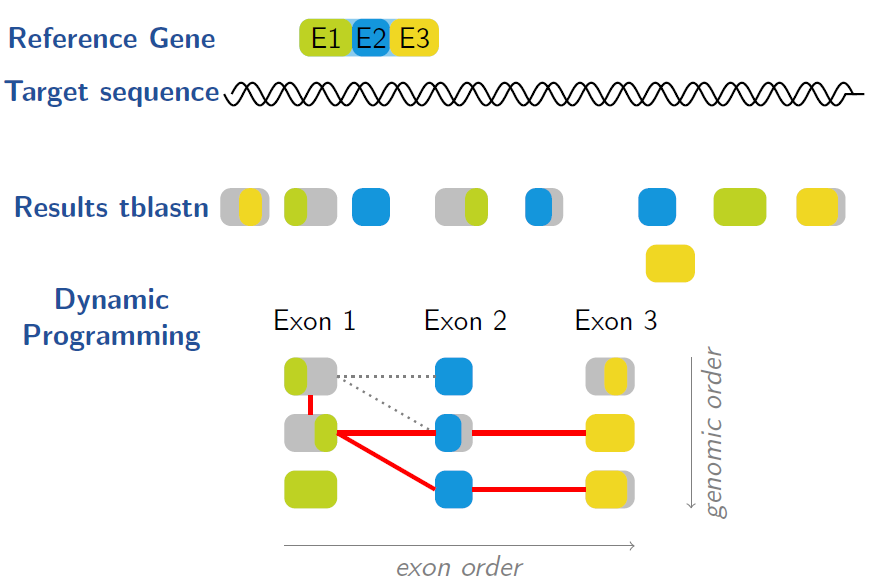
\includegraphics[width=\linewidth]{schema}
\caption{Illustration of the GeMoMa algorithm. GeMoMa uses \texttt{tblastn} to search for homologs of all (partially) coding exons of the reference transcript. Subsequently, a dynamic programming algorithm is used to determine the best combination of the hits.}
\end{figure}

\clearpage

\section{GeMoMa in a nutshell}

There are 6 essential steps that are divided into 3 phases. However, if you do not have any RNA-seq data you can skip the first phase.
This guide only provides a rough overview. If your are interested in individual parameters you can call:
\begin{verbatim}
java -jar GeMoMa-<version>.jar CLI <toolname>
\end{verbatim}
which will provide descriptions of all available parameters.

Keep in mind that homology-based gene prediction only allows us to infer genes with known peers in at least one reference organism. Hence, homology based gene prediction might miss genes with no known peer in the reference organism(s), even if these are expressed in the RNA-seq data. On the other hand, homology-based gene prediction allows for inferring genes that are not or rarely expressed in the RNA-seq samples.

\begin{figure}[h]
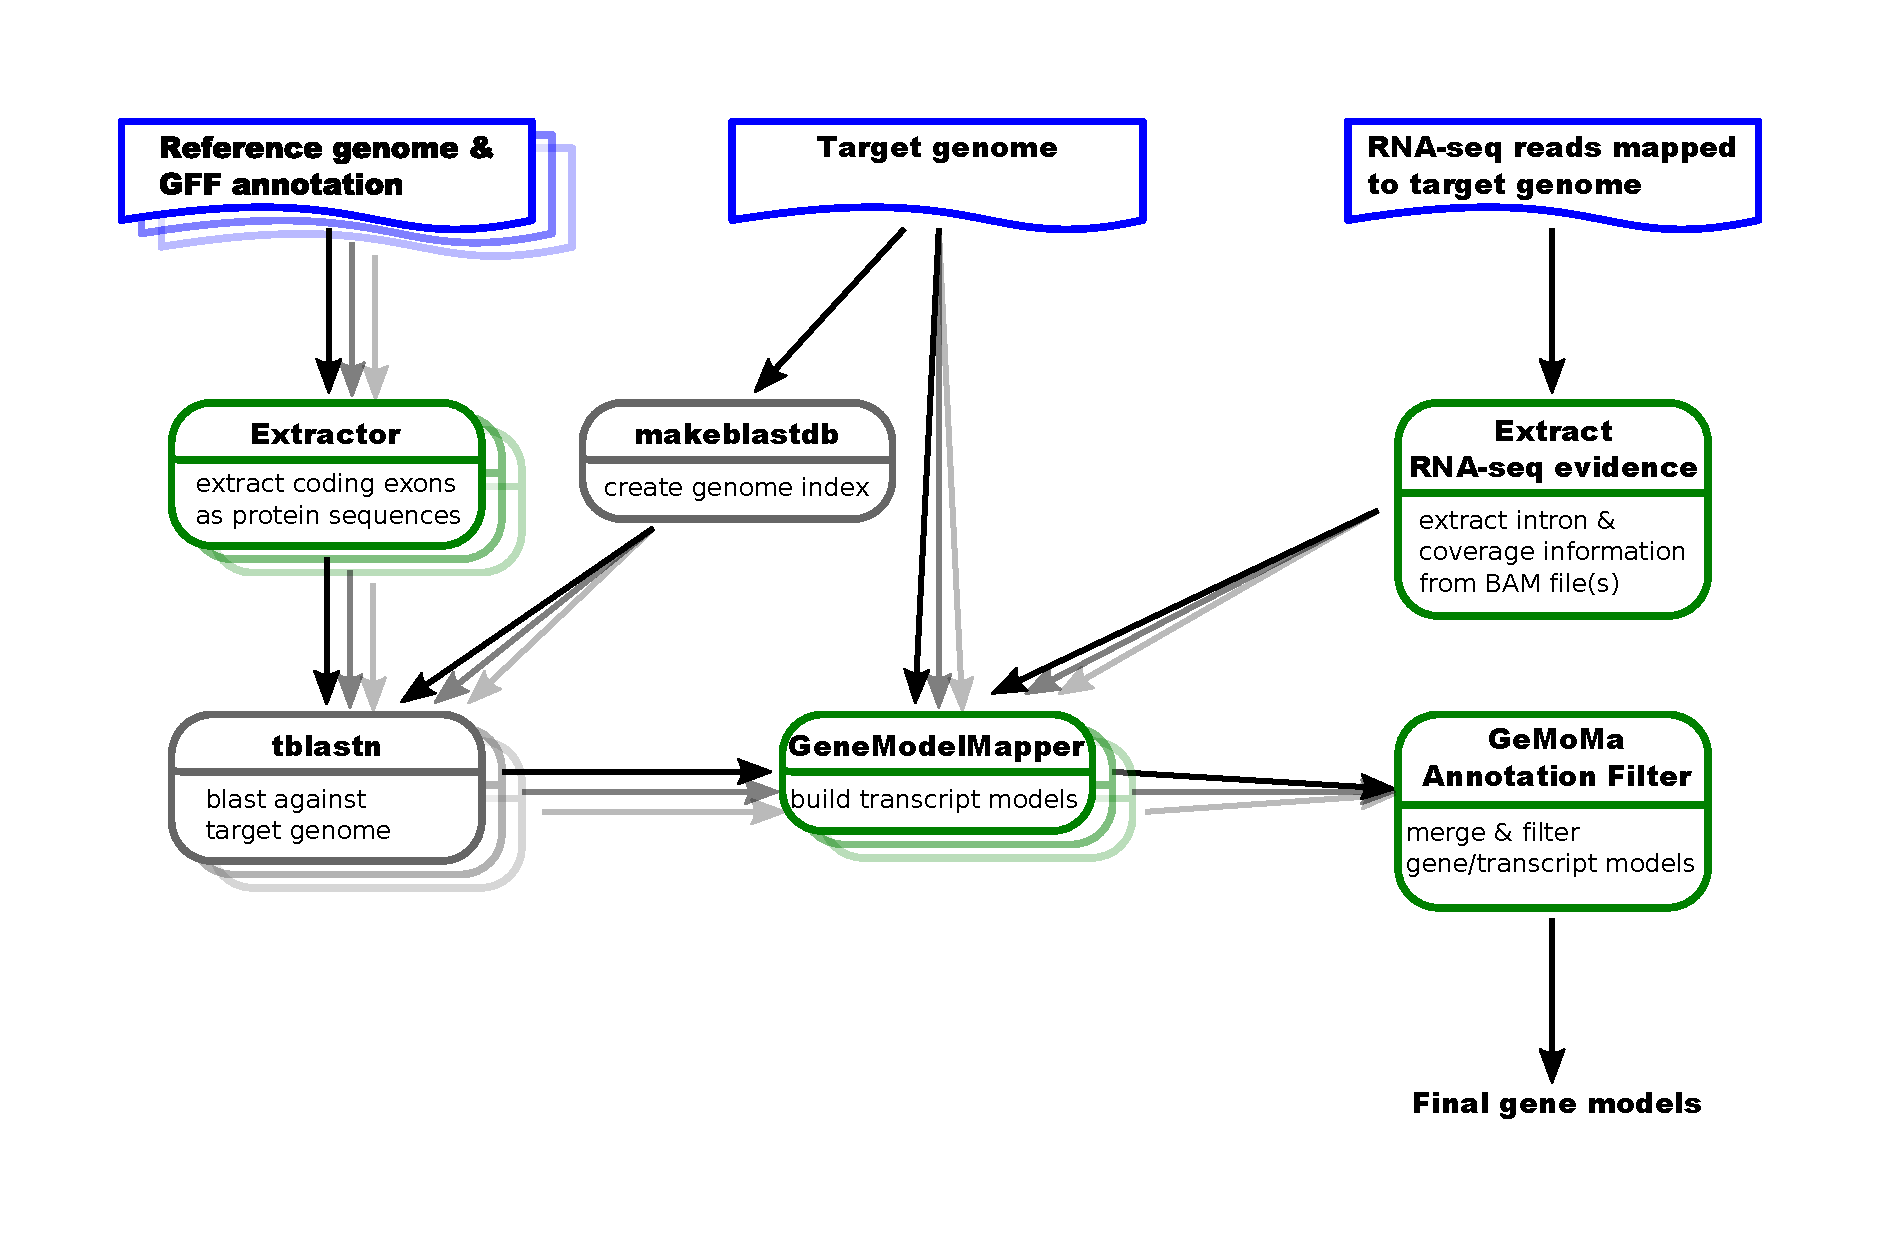
\includegraphics[width=\linewidth]{drawing.pdf}
\caption{GeMoMa workflow. Blue items represent input data sets, green boxes represent GeMoMa modules, while grey boxes represent external modules. The GeMoMa Annotation Filter allows to combine predictions from different reference species and produces the final output. RNA-seq data is optional.}
\end{figure}

\clearpage

\subsection{Quick start}
We provide two scripts:
\begin{enumerate}
	\item A test script checking whether GeMoMa runs on your system on some tiny toy data: \texttt{test\_without\_RNAseq.sh}. Example data (input and output) can be found in directory \texttt{test\_data}.
	\item An application script allowing to start the complete GeMoMa workflow with minimal parameter input: \texttt{run.sh}. If you like to run GeMoMa with standard parameters and without any tricks for speed up you can just use this script.
\begin{itemize}
	\item Without RNA-seq data:
\begin{verbatim}
./run.sh <ref-anno> <ref-genome> <target-genome> <out-dir>
\end{verbatim}	
	\item With RNA-seq data:
\begin{verbatim}
./run.sh <ref-anno> <ref-genome> <target-genome> <out-dir>
         <lib-type> <mapped-reads>
\end{verbatim}
\end{itemize}
where
\begin{enumerate}
	\item \texttt{ref-anno} is the annotation of the reference organism (GFF/GTF)
	\item \texttt{ref-genome} is the genome of the reference organism (FastA)
	\item \texttt{target-genome} is the genome of the target organism (FastA)
	\item \texttt{out-dir} is the output directory
	\item \texttt{lib-type} is the RNA-seq library type\\
		(\verb"{FR_UNSTRANDED, FR_FIRST_STRAND, FR_SECOND_STRAND}")
	\item \texttt{mapped-reads} are the mapped RNA-seq reads (SAM/BAM)
\end{enumerate}
\end{enumerate}

\clearpage

\subsection{Phase 1: Preprocessing RNA-seq data}
For this phase, you need RNA-seq data and a reference sequence or assembly of your target organism.
This allows for inferring experimental verified introns and coverage. In the following command lines ''\verb"..."`` should be replaced by your specific parameters.

\begin{enumerate}
\item	Run your favorite read mapper (e.g. TopHat, \ldots) on your RNA-seq data
\item	Extract introns (and coverage) running: 
\begin{verbatim}
java -jar GeMoMa-<version>.jar CLI ERE ...
\end{verbatim}
\end{enumerate}

\subsection{Phase 2: Prediction candidate transcripts}
For this phase, you need at least one reference organism with reference sequence/assembly and annotation as well as a reference sequence/assembly for the target organism.
Keep in mind that the outcome of GeMoMa highly depends on the quality of the reference annotation.
It is possible to run step 3 to 5 with multiple reference organisms.

\begin{enumerate}
\setcounter{enumi}{2}
\item Extract CDS-parts (and proteins) of the reference organism running:
	\begin{verbatim}
	java -jar GeMoMa-<version>.jar CLI Extractor...
	\end{verbatim}
\item Find homologous parts in the target organism running: 
	\begin{verbatim}
	tblastn -outfmt "6 std sallseqid score nident positive gaps
	         ppos qframe sframe qseq sseq qlen slen salltitles" ...
	\end{verbatim}
	The output format of tblastn is essential for GeMoMa.
\item Find homologous candidate transcripts in the target organism running:
	\begin{verbatim}
	java -jar GeMoMa-<version>.jar CLI GeMoMa ...
	\end{verbatim}
	Since version 1.4, p=10 and ct=0.4 are new default values.
\end{enumerate}

\subsection{Phase 3: Aggregate and filter predictions}
For this phase, you need only the output of step 5.
If you ran the second phase for multiple reference organisms, the individual predictions can now be combined in this step.

\begin{enumerate}
\setcounter{enumi}{5}
\item Aggregate predictions running: 
\begin{verbatim}
java -jar GeMoMa-<version>.jar CLI GAF ...
\end{verbatim}
\end{enumerate}

\clearpage
\section{Miscellaneous}

\subsection{Help section and parameter description}
If you like to receive more information about the available tools and parameters please enter
\begin{verbatim}
java -jar GeMoMa-<version>.jar CLI
\end{verbatim}
and follow the instructions.

\subsection{General speed-up}
If you
\begin{enumerate}
\item like to speed-up the computation,
\item have lots of compute cores and
\item have large data set (i.e., a large number of lines in the CDS-parts file),
\end{enumerate}
you can split the job in several independent jobs. Splitting the job can be done using
\begin{verbatim}
java -cp GeMoMa-<version>.jar projects.FastaSplitter <CDS-parts> 
     <numberOfSplits> "_"
\end{verbatim}

This will result in several independent FastA files containing some CDS-parts. You can run steps 4 and 5 on these individual parts.
Finally, you have to concatenate the resulting predicted annotations, protein, \ldots before starting step 6.

\subsection{Genome-wide vs. specific genes}
By default, GeMoMa tries to make predictions for all CDS of the reference organism in the target organism. Hence, we call this a genome-wide approach. Additionally, Extractor and GeMoMa have an option for filtering based on a list of some reference CDS (cf. parameter \texttt{selected}). This approach allows to further speed up the predictions especially if one is interested only in a certain part of the annotation.

\subsection{Galaxy integration}
GeMoMa provides a command line interface as well as everything to be integrated in your local Galaxy instance. For creating the XML files that are needed for integration into Galaxy, just run: 
\begin{verbatim}
createGalaxyIntegration.sh <version>
\end{verbatim}

Alternatively, you can run the individual commands on your own using the command line
\begin{verbatim}
java -jar GeMoMa-<version>.jar --create
\end{verbatim}
If you like to modify some VM arguments for the java calls made by Galaxy you can alter them for each sub-tool individually. If you like to allow GeMoMa to allocate at most 40GB of RAM, you may do so by running
\begin{verbatim}
java -jar GeMoMa-<version>.jar --create GeMoMa -Xmx40g
\end{verbatim}
to create the corresponding XML integration for GeMoMa.

\section{Reference, questions and comments}
If you use GeMoMa please cite:\\
\emph{Using intron position conservation for homology-based gene prediction.}\\
J. Keilwagen, M. Wenk, J. L. Erickson, M. H. Schattat, J. Grau, and F. Hartung.
Nucleic Acids Research, 2016. doi: \href{https://doi.org/10.1093/nar/gkw092}{10.1093/nar/gkw092}\\
~\\
FAQs, complete parameter lists, release notes, \ldots can be found on the homepage: 
\url{http://www.jstacs.de/index.php/GeMoMa}\\
~\\
For further questions or comments, please contact:\\
\href{mailto:jens.keilwagen@julius-kuehn.de?subject=GeMoMa manual}{jens.keilwagen@julius-kuehn.de}
\end{document}